\documentclass[11pt]{article}

\usepackage[margin=1in]{geometry}
\usepackage{graphicx}
\usepackage{booktabs}
\usepackage{hyperref}
\usepackage{amsmath}
\usepackage{xcolor}

\title{Can a CNN Learn Snake in a Hallucinated Environment?\\
\large A Small-Scale Study of Visual World-Model Exploitation and Grounding}
\author{Anonymous}
\date{}

\begin{document}
\maketitle

\begin{abstract}
Interactive video world models suggest a route to training agents without querying the true environment at every step.
This paper studies a deliberately small version of that problem: train an action-conditioned visual world model for Snake, train CNN policies only inside that learned model, and evaluate the resulting policies in the true code simulator.
The experiment is designed to expose transfer gaps and model-exploitation behavior rather than hide them.
The world model predicts the next RGB frame, scalar reward, death probability, and an unclamped floating-point snake length from a short visual context and an action.
The rendered frame contains only the game board; reward, episode end, and snake length are predicted as separate scalar outputs.
We report hallucinated return, real-simulator return, and their gap across world-model scale, context length, and CNN policy size.
We also evaluate an iterative grounding loop in which a policy trained inside the world model generates action traces, those traces are replayed in the true simulator to collect correct visual transitions, and the existing world model is fine-tuned rather than retrained from scratch.
\end{abstract}

\section{Introduction}
Generative interactive environments such as Genie~\cite{bruce2024genie} and real-time streaming game world models such as Matrix-Game 2.0~\cite{he2025matrixgame2} make it plausible to use learned video dynamics as training environments.
For reinforcement learning, however, a learned environment is also an attack surface: if the policy can discover model inaccuracies that produce reward inside the model but do not transfer to the real environment, apparent progress can be negative transfer.

We study this question in Snake because the true simulator is cheap, deterministic, and unambiguous.
That lets us measure the gap between imagined performance and real performance without arguing about evaluator noise.
The core question is not whether Snake can be solved by a CNN.
It can.
The question is narrower: when a CNN policy is trained only against a learned visual dynamics model, does it learn behavior that transfers back to the real simulator, or does it exploit the model?

\section{Method}
\paragraph{Environment.}
The simulator renders a $128 \times 128 \times 3$ RGB Snake board.
The image contains just the game: checkerboard board, rocks, apples, and snake.
There is no HUD, score text, keyboard overlay, or extra visual marker for death or win.
Episode status is supervised separately: the world model predicts scalar reward, whether the episode has ended, and snake length through non-visual heads.

\begin{figure}[t]
  \centering
  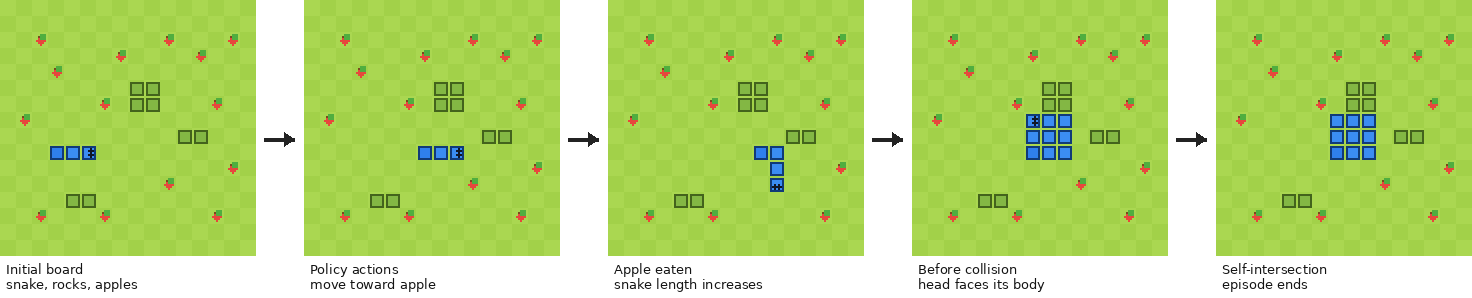
\includegraphics[width=\linewidth]{figures/snake_environment_sequence.png}
  \caption{Simulator-only environment sequence. The frames show the initial board, movement toward an apple, eating an apple, and a self-intersection episode ending. These images come from the true simulator, not the learned world model.}
  \label{fig:environment-sequence}
\end{figure}

\paragraph{World model.}
The world model is action-conditioned and autoregressive.
Given the previous $k \in \{1,2,5\}$ frames, previous reward, and the next discrete action, it predicts:
\begin{equation}
  \hat{x}_{t+1},\quad \hat{r}_{t+1},\quad \hat{d}_{t+1},\quad \hat{\ell}_{t+1}
\end{equation}
where $\hat{x}_{t+1}$ is the next RGB frame, $\hat{r}_{t+1}$ is scalar reward, $\hat{d}_{t+1}$ is a death logit, and $\hat{\ell}_{t+1}$ is a floating-point snake length prediction.
The length output is intentionally not clamped, so large or implausible deviations remain measurable.
The model always predicts only one next frame at a time.
The context length $k$ controls how many past frames are given as input: $k=1$ is the previous-frame-only setting, while $k=2$ and $k=5$ test whether short visual history helps the model infer recent motion, action effects, and autoregressive rollout stability.
Although a single Snake frame contains most of the board state, extra context may still help because the simulator handles direction-dependent actions such as ignored reverse moves.

\paragraph{Policy training.}
For each frozen world model, CNN policies of three sizes are trained with PPO~\cite{schulman2017ppo} inside hallucinated rollouts.
Episodes in the learned environment end when the predicted death probability crosses a threshold or when the rollout reaches a maximum length.
Policies are then evaluated in both the learned world model and the true simulator.

\paragraph{Scalar objective ablation.}
Snake has a useful internal consistency check: the initial snake length is 3, and under the raw apple reward the true length after a rollout equals $3 + \sum_t r_t$.
We therefore compare two model-derived length estimates: the direct floating-point length head $\hat{\ell}_t$, and the reward-integrated estimate $3 + \sum_t \hat{r}_t$.
This diagnostic does not decide which signal PPO should optimize; it only checks which scalar is more numerically consistent with real simulator length under fixed actions.
We then freeze one world model checkpoint and train otherwise identical medium CNN policies with three PPO objectives: predicted reward, predicted length change $\hat{\ell}_{t+1}-\hat{\ell}_t$, and a mixed objective.
This separates scalar prediction quality from policy-transfer performance.

\paragraph{Grounding loop.}
The grounding experiment is designed to approximate settings where real data are expensive but not impossible to obtain.
After training a policy inside the world model, we execute that policy's actions in the real simulator, collect a small set of correct transitions, merge those transitions with the original random/safe/greedy dataset, and fine-tune the existing world model checkpoint.
We repeat this loop several times and measure whether the hallucinated-real return gap shrinks.
This is closer to deployment-time grounding than training a new model from scratch on policy-generated data.
Ignoring initial pretraining, each grounding round collects at most 1000 new real simulator transitions before policy training resumes.
At 30 frames per second, 1000 transitions correspond to roughly 0.56 minutes of newly collected real data.
The following policy-training phase uses 300 PPO updates with 32 learned environments and 64 rollout steps, or 614{,}400 imagined transitions.
This corresponds to roughly 614 imagined transitions per new real transition when the collection cap is reached.
One completed round collected fewer transitions because the policy episodes ended early, so its imagined/real ratio is larger.

\section{Experimental setup}
The main dataset contains 50,000 real simulator transitions from a mixture of random, safe-random, straight, and greedy policies.
The main sweep trains two world-model sizes, three context lengths, and three CNN policy sizes, yielding 18 world-model/policy settings.
The public W\&B report is linked from the accompanying repository.

\begin{figure}[t]
  \centering
  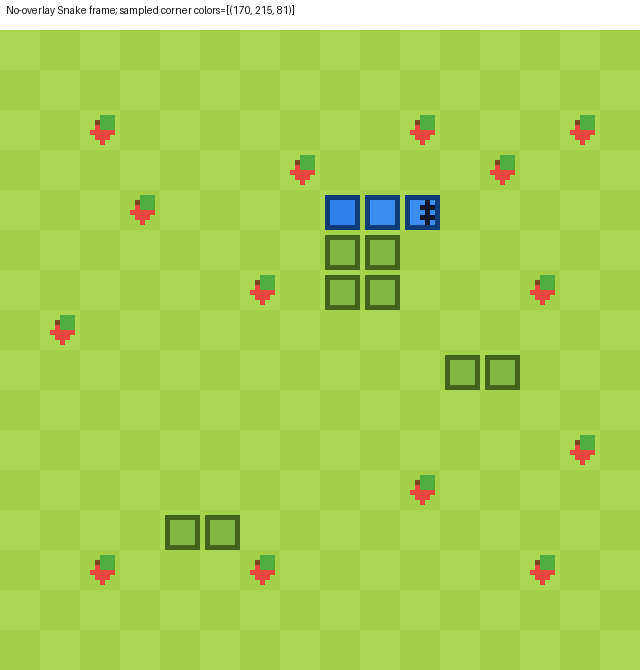
\includegraphics[width=0.55\linewidth]{figures/snake_simulator_frame.png}
  \caption{Example simulator frame. The rendered image contains the game board, rocks, apples, and snake. Episode status and reward are not written into the image.}
  \label{fig:example-frame}
\end{figure}

\section{Results}
The tables and plots in this section are generated from the synced experiment artifacts by the repository's artifact-export script.

\begin{table}[t]
  \centering
  \begin{tabular}{lllrrrr}
\toprule
WM & Ctx & CNN & Hall. & Real & Gap & Apples \\
\midrule
wm\_2m & 5 & small & 7.401 & 6.000 & 1.401 & 6.000 \\
wm\_1m & 1 & small & 0.395 & -1.000 & 1.395 & 0.000 \\
wm\_1m & 1 & large & 0.356 & -1.000 & 1.356 & 0.000 \\
wm\_2m & 5 & medium & 5.469 & 6.000 & -0.531 & 6.000 \\
wm\_2m & 1 & small & -1.904 & -1.000 & -0.904 & 0.000 \\
wm\_1m & 1 & medium & -1.980 & -1.000 & -0.980 & 0.000 \\
wm\_2m & 1 & large & -2.410 & -1.000 & -1.410 & 0.000 \\
wm\_1m & 2 & large & 7.529 & 9.000 & -1.471 & 10.000 \\
wm\_1m & 2 & small & 4.950 & 7.000 & -2.050 & 8.000 \\
wm\_2m & 1 & medium & -3.105 & -1.000 & -2.105 & 0.000 \\
wm\_1m & 5 & small & 8.927 & 12.000 & -3.073 & 12.000 \\
wm\_1m & 5 & medium & 7.877 & 11.000 & -3.123 & 12.000 \\
wm\_1m & 2 & medium & 6.908 & 12.000 & -5.092 & 12.000 \\
wm\_2m & 2 & large & 10.120 & 18.000 & -7.880 & 13.000 \\
wm\_2m & 5 & large & 8.831 & 18.000 & -9.169 & 13.000 \\
wm\_2m & 2 & medium & 8.481 & 18.000 & -9.519 & 13.000 \\
wm\_1m & 5 & large & 7.749 & 18.000 & -10.251 & 13.000 \\
wm\_2m & 2 & small & 7.521 & 18.000 & -10.479 & 13.000 \\
\bottomrule
\end{tabular}

  \caption{Main transfer results. Gap is hallucinated return minus real-simulator return; a positive gap indicates the policy performed better inside the world model than in the true simulator.}
  \label{tab:main-results}
\end{table}

\begin{figure}[t]
  \centering
  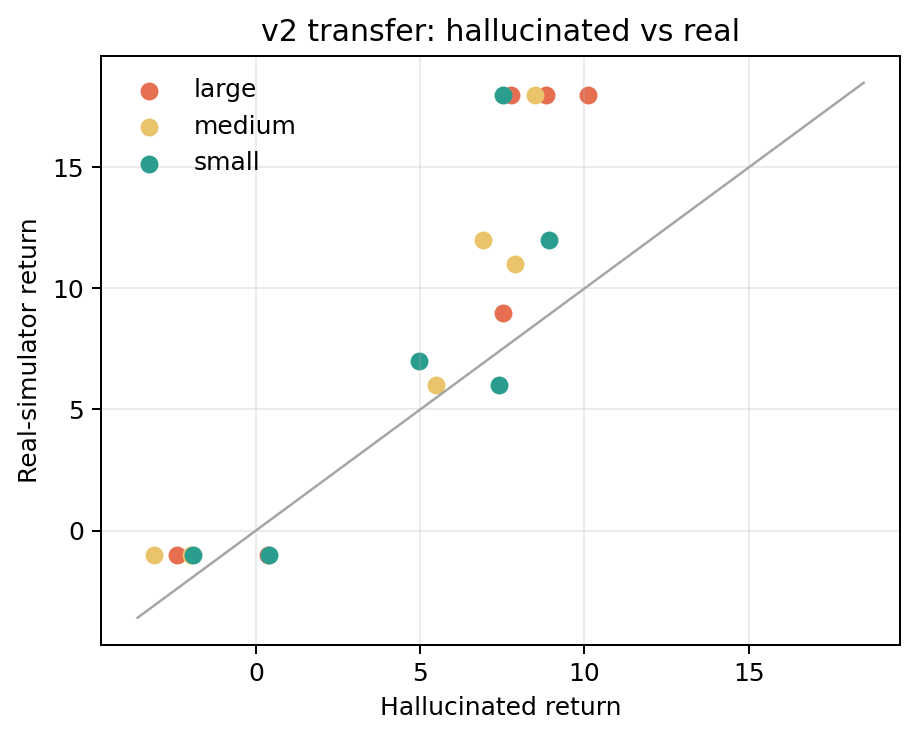
\includegraphics[width=0.75\linewidth]{figures/hallucinated_vs_real.png}
  \caption{Hallucinated return versus real-simulator return. The diagonal marks equal return. Points below the diagonal have hallucinated return greater than real return, while points above the diagonal transfer better than the model predicted.}
  \label{fig:hallu-real}
\end{figure}

\begin{figure}[t]
  \centering
  
\includegraphics[width=\linewidth]{figures/wm_vs_sim_rollout.png}
  \caption{Autoregressive world-model rollout against simulator frames. The difference row visualizes pixel-level drift.}
  \label{fig:rollout}
\end{figure}

\begin{figure}[t]
  \centering
  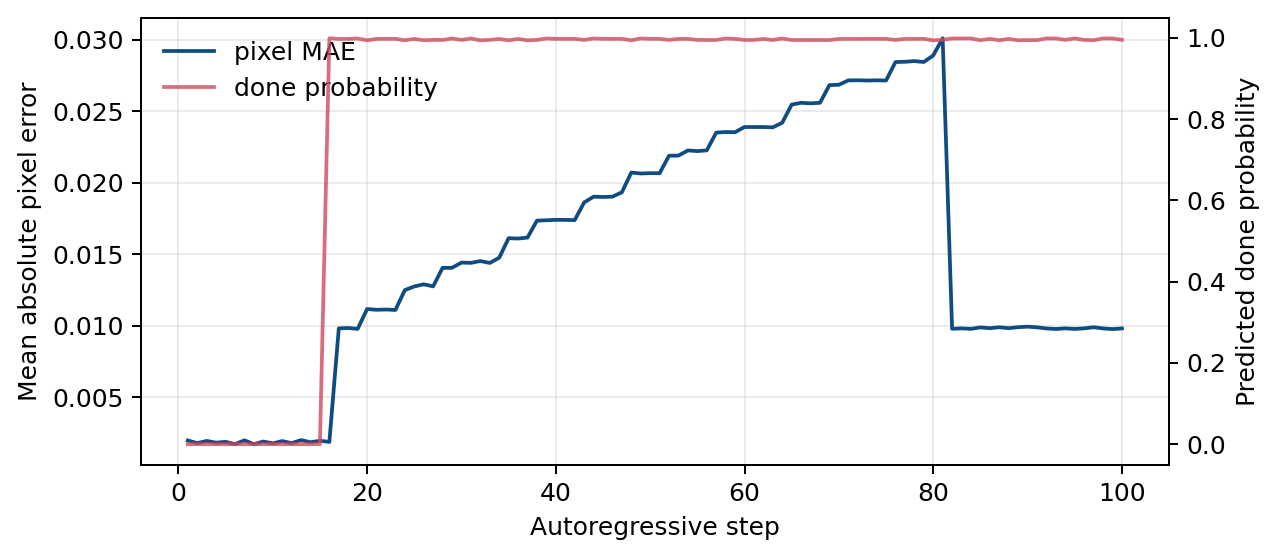
\includegraphics[width=0.8\linewidth]{figures/wm_drift_curve.png}
  \caption{Pixel error and predicted terminal probability across an autoregressive rollout.}
  \label{fig:drift}
\end{figure}

\begin{table}[t]
  \centering
  \begin{tabular}{rrrrrrrr}
\toprule
Iter. & New trans. & Real min & Imag. trans. & Imag./real & Hall. & Real & Gap \\
\midrule
1 & 1000 & 0.556 & 614400 & 614.4 & -0.024 & -1.000 & 0.976 \\
2 & 440 & 0.244 & 614400 & 1396.4 & -8.300 & 0.000 & -8.300 \\
3 & 1000 & 0.556 & 614400 & 614.4 & 1.073 & 0.000 & 1.073 \\
\bottomrule
\end{tabular}

  \caption{Iterative grounding results. Each iteration collects a small amount of real simulator data using the previous policy's actions, fine-tunes the existing world model, and then trains the policy inside the updated fixed world model. Real-data minutes assume 30 FPS.}
  \label{tab:grounding}
\end{table}

\begin{table}[t]
  \centering
  \begin{tabular}{lrr}
\toprule
Metric & Length head & Reward-integrated \\
\midrule
Step MAE & 2.039 & 1.158 \\
Step median AE & 1.491 & 0.545 \\
Apple-step MAE & 2.562 & 1.740 \\
Better step fraction & 0.124 & 0.876 \\
Better episode count & 86.000 & 114.000 \\
\bottomrule
\end{tabular}

  \caption{Scalar consistency diagnostic on a fixed world model. The reward-integrated estimate is $3 + \sum_t \hat{r}_t$ and is compared against true simulator snake length. Lower error is better.}
  \label{tab:scalar-consistency}
\end{table}

\begin{figure}[t]
  \centering
  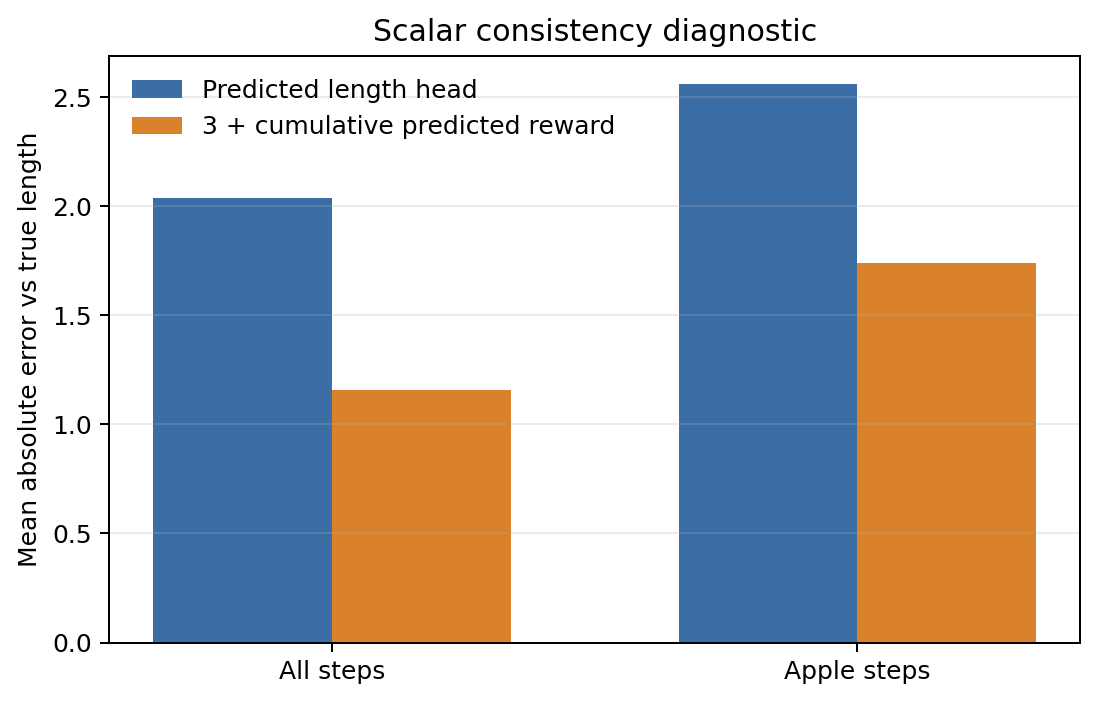
\includegraphics[width=0.72\linewidth]{figures/scalar_consistency_mae.png}
  \caption{Direct length-head error versus reward-integrated length error. This diagnostic asks which scalar output better tracks true length under fixed action rollouts; it does not by itself establish which signal is better for PPO.}
  \label{fig:scalar-consistency-mae}
\end{figure}

\begin{figure}[t]
  \centering
  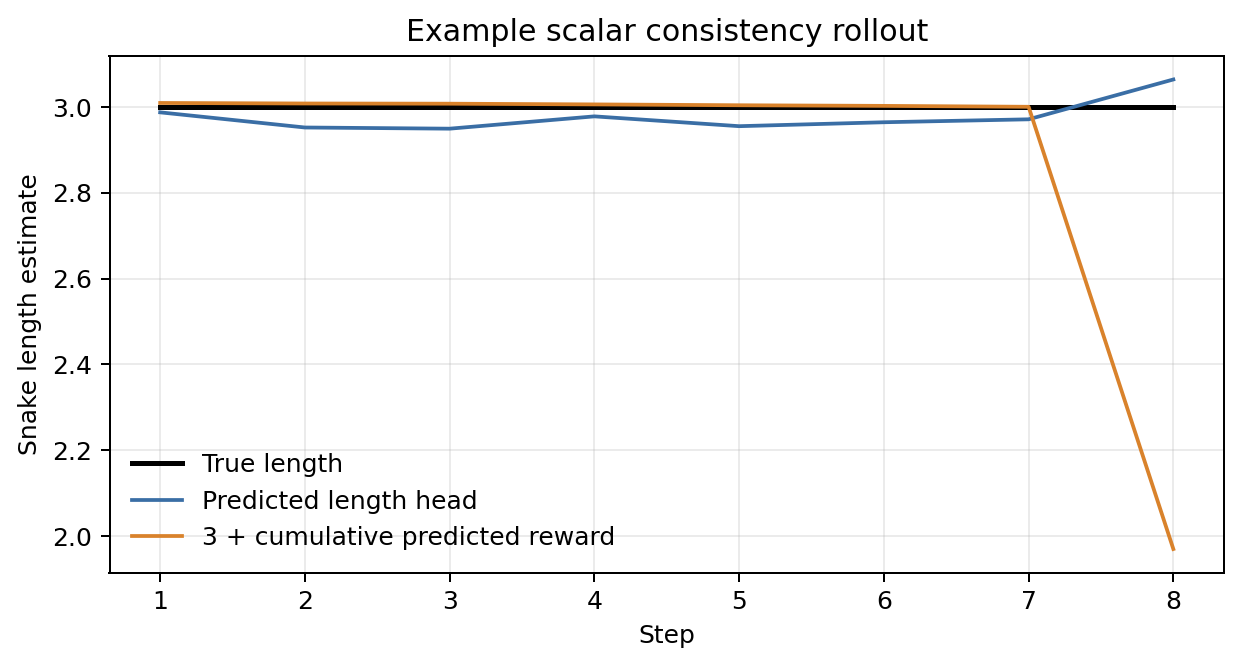
\includegraphics[width=0.78\linewidth]{figures/scalar_consistency_rollout.png}
  \caption{Example scalar rollout comparing true length, the direct length head, and $3 + \sum_t \hat{r}_t$. Counterexamples exist, so the result should be read as an average diagnostic rather than an invariant.}
  \label{fig:scalar-consistency-rollout}
\end{figure}

\begin{table}[t]
  \centering
  \begin{tabular}{lrrrr}
\toprule
Objective & Hall. & Real & Apples & Death rate \\
\midrule
Predicted reward & 3.576 & 1.000 & 2.000 & 1.000 \\
Length change & 1.136 & 0.000 & 1.000 & 1.000 \\
Mixed & 2.076 & 0.000 & 1.000 & 1.000 \\
\bottomrule
\end{tabular}

  \caption{Fixed-world-model PPO objective ablation. The world model checkpoint and policy size are held fixed while PPO optimizes predicted reward, predicted length change, or a mixed scalar objective.}
  \label{tab:reward-objective}
\end{table}

\begin{figure}[t]
  \centering
  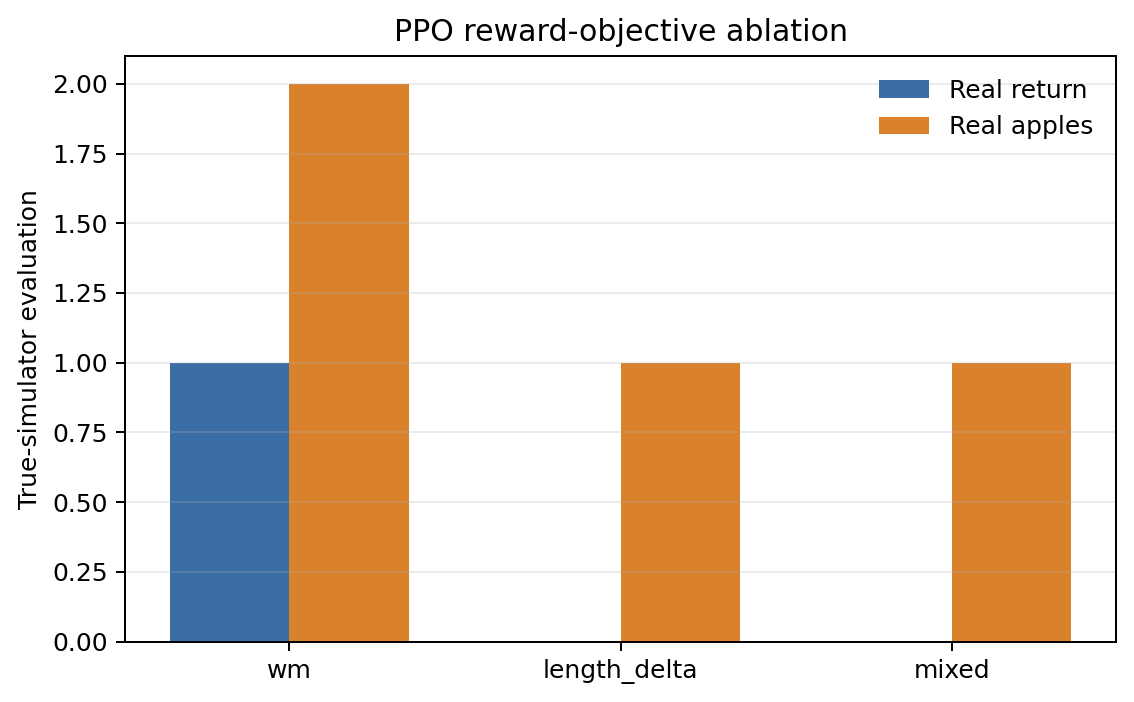
\includegraphics[width=0.72\linewidth]{figures/reward_objective_ablation.png}
  \caption{True-simulator performance after PPO training under different scalar objectives inside the same fixed world model. This is the direct test of whether a scalar that is numerically accurate also helps policy transfer.}
  \label{fig:reward-objective}
\end{figure}

\section{Discussion}
This study is intentionally small, but the exploitation mechanism is the point.
If a CNN trained inside a learned Snake model obtains positive hallucinated return and negative real return, then the learned environment is not just inaccurate; it is exploitable by the policy optimizer.
The most important quantity is therefore not frame MAE alone, but the transfer gap between imagined and real returns.

The grounding loop tests a practical mitigation.
If the policy finds a model exploit, replaying its actions in the true simulator reveals the correct transitions near that exploit.
Fine-tuning the world model on a small number of these transitions should, in principle, make the exploit harder to repeat.
We use discrete grounding rounds rather than continuously updating the world model during PPO, because a fixed learned environment makes the transfer gap easier to interpret.
In a more expensive real-world setting, the relevant budget is the ratio of imagined PPO transitions to newly collected real transitions: one can train for many simulated steps per hour of real data, but excessive policy optimization between grounding rounds may increase model exploitation.
The experiment does not prove that this scales to humanoids or open-world games.
It provides a controlled measurement harness for the same mechanism: train in imagination, evaluate in reality, then ground the model where the policy drove it out of distribution.

\section{Limitations}
Snake is discrete, low-dimensional, and rendered from complete state.
The results should not be interpreted as evidence that small CNN policies or small latent world models are sufficient for richer domains.
The dataset is also policy-biased; random/safe/greedy trajectories do not cover every state that a trained optimizer may induce.
Finally, the current experiments use a single simulator and a modest compute budget, so conclusions should be framed as a reproducible case study rather than a general scaling law.

\section{Reproducibility}
The code, configs, generated figures, and selected result artifacts are packaged in the accompanying repository.
The main config and local smoke test are included in the accompanying repository.
Experiment metrics are logged to the linked W\&B project.

\bibliographystyle{plain}
\bibliography{references}
\end{document}
